\section{An included file}
Text from an included file. Its main file is found automatically because main.tex inputs it.

\newpage
\section{A drawing}
TikZ pictures are drawn natively. Editing their labels keeps the drawing and label rotation.

\begin{center}
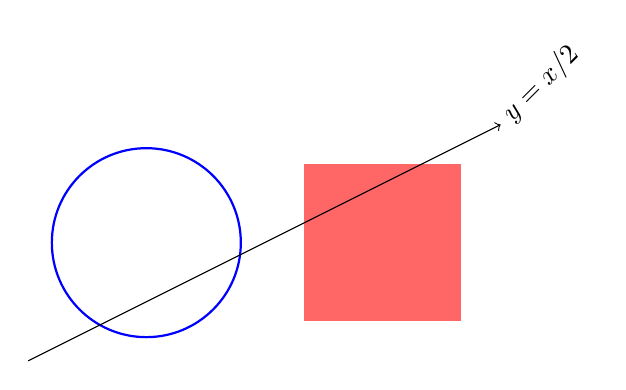
\begin{tikzpicture}
  \draw[thick,blue] (0,0) circle (1.2);
  \fill[red!60] (2,-1) rectangle (4,1);
  \draw[->] (-1.5,-1.5) -- (4.5,1.5) node[right,rotate=45] {$y = x/2$};
\end{tikzpicture}
\end{center}
